\documentclass[a4paper,12pt]{article}
\usepackage[utf8]{inputenc}
\usepackage[spanish]{babel}
\usepackage{color}
\usepackage{parskip}
\usepackage{graphicx}
\usepackage{multirow}
\usepackage{listings}
\usepackage{vmargin}
\usepackage{datetime}
\newdate{date}{07}{12}{2017}
\graphicspath{ {imagenes/} }
\definecolor{mygreen}{rgb}{0,0.6,0}
\definecolor{lbcolor}{rgb}{0.9,0.9,0.9}
\usepackage{epstopdf}
\usepackage{float}


\setpapersize{A4}
\setmargins{2.5cm}       % margen izquierdo
{1.5cm}                        % margen superior
{16.5cm}                      % anchura del texto
{23.42cm}                    % altura del texto
{10pt}                           % altura de los encabezados
{1cm}                           % espacio entre el texto y los encabezados
{0pt}                             % altura del pie de página
{2cm}     

\lstset{
    tabsize=4,    
%   rulecolor=,
    language=[GNU]C++,
        basicstyle=\tiny,
        aboveskip={1.5\baselineskip},
        columns=fixed,
        showstringspaces=false,
        extendedchars=false,
        breaklines=true,
        prebreak = \raisebox{0ex}[0ex][0ex]{\ensuremath{\hookleftarrow}},
        frame=single,
        showtabs=false,
        showspaces=false,
        showstringspaces=false,
        identifierstyle=\ttfamily,
        keywordstyle=\color[rgb]{0,0,1},
        commentstyle=\color[rgb]{0.026,0.112,0.095},
        stringstyle=\color{red},
        numberstyle=\color[rgb]{0.205, 0.142, 0.73},
%        \lstdefinestyle{C++}{language=C++,style=numbers}’.
}


\begin{document}
\title{Ejercicio del Examen}
\author{
Christofer Fabián Chávez Carazas \\
\small{Universidad Nacional de San Agustín de Arequipa} \\
\small{Escuela Profesional de Ciencia de la Computación} \\
\small{Compiladores}
}
\date{\displaydate{date}}

\maketitle

\begin{large}
 \textbf{Problema}
\end{large}

Hacer un programa que detecte todas las coincidencias de un patron en una cadena dada.

\begin{large}
 \textbf{Codigo}
\end{large}

Dentro de un vertor se guardan todas las posibles coincidencias, y se va verificando cada una hasta que sea aceptada, o no sea igual al patron en un caracter,
lo cual hace que se borre del vector.

\begin{lstlisting}
#include <iostream>
#include <vector>

using namespace  std;

class Cadena{
public:
	Cadena(int size, int posIni){
		cadena = "";
		actual = 0;
		for(int i = 0; i < size; i++){
			cadena.push_back('-');
		}
		this->posIni = posIni;
		aceptada = false;
	}
	void pushCharacter(char c){
		cadena[actual] = c;
		actual++;
	}
	bool verifyCharacter(string patron, char c){
		if(cadena.back() != '-'){
			aceptada = true;
			return true;
		} 
		if(patron[actual] == c){
			pushCharacter(c);
			return true;
		} 
		return false;
	}
	bool verifyCadena(){
		for(char c : cadena){
			if(c == '-') return false;
		}
		return true;
	}
	int actual;
	int posIni;
	bool aceptada;
	string cadena;
};

vector<Cadena> getPatron(string patron, string cadena){
	vector<Cadena> res;
	for(int i = 0; i < cadena.size(); i++){
		char c = cadena[i];
		for(int j = 0; j < res.size(); j++){
			if(res[j].verifyCharacter(patron, c) == false){
				res.erase(res.begin() + j);
				j--;
			}
		}
		if(c == patron[0]){
			res.push_back(Cadena(patron.size(), i));
			res.back().pushCharacter(c);
		}
	}
	for(int i = 0; i < res.size(); i++){
		if(res[i].verifyCadena() == false){
			res.erase(res.begin() + i);
			i--;
		}
	}
	return res;
}

int main(){
	string patron;
	string cadena;
	cout<<"Escriba la cadena:";
	cin>>cadena;
	cout<<"Escriba el patron:";
	cin>>patron;
	vector<Cadena> res = getPatron(patron, cadena);
	cout<<"Se encontraron "<<res.size()<<" coincidencias"<<endl;
	for(Cadena cad : res){
		cout<<"Posicion->"<<cad.posIni<<endl;
	}
}
\end{lstlisting}

\begin{figure}[H]
 \centering
 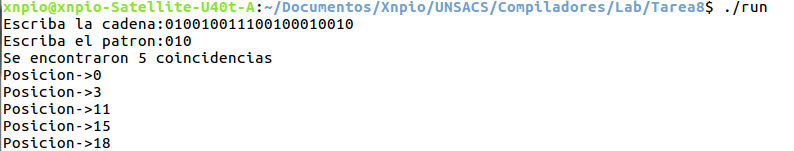
\includegraphics[scale = 0.5]{1.png}
\end{figure}
\begin{figure}[H]
 \centering
 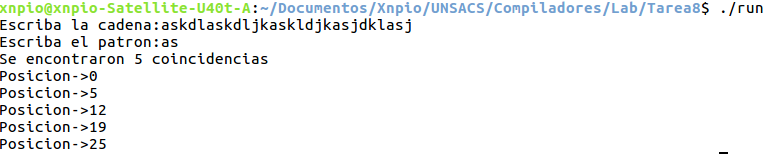
\includegraphics[scale = 0.5]{2.png}
 \caption{Resultados del programa}
\end{figure}






\end{document}

